
\chapter{Getting meteorological data}\label{app:GettingMetData}

	\begin{onehalfspace}
	
		%	Formato con ejemplo y capturas:
		
		\section{Getting an annual text file from NDBC}

			The following steps shows the procedure to obtain an annual text file that contain the measurements collected by a buoy from NDBC, concretely the file of the year $2017$ corresponding to the buoy identified as \textit{Station 46001}, moored at Western Gulf of Alaska.
			
				\begin{itemize}
					%\setlength\itemsep{0.01cm}
					\item \textit{\textbf{Step 1}}: Open the web browser and visit the NDBC web page \cite{NOAA_1}.
					\item \textit{\textbf{Step 2}}: Navigate to the desired buoy and click on the year to download (see Fig. \ref{fig:selectingBuoy}).
						\begin{figure}[ht!]
							\centering
							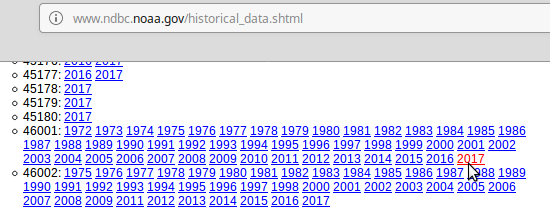
\includegraphics[scale=0.48]{figures/selectingBuoy.png}
							\caption{Selecting the desired buoy and year.}
							\label{fig:selectingBuoy}
						\end{figure}
					\item \textit{\textbf{Step 3}}: In the option \textit{\textbf{Method Two}} click on the file (see Fig. \ref{fig:downloadingTextFile}) and its content will be shown.
						\begin{figure}[ht!]
							\centering
							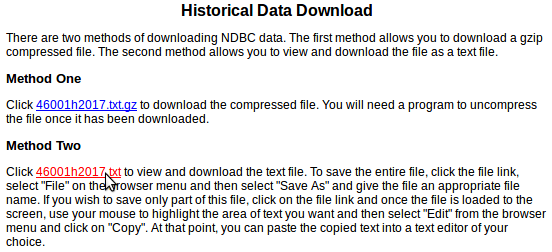
\includegraphics[scale=0.48]{figures/downloadingTextFile.png}
							\caption{Downloading the annual text file.}
							\label{fig:downloadingTextFile}
						\end{figure}
					\item \textit{\textbf{Step 4}}: In the menu bar of the web browser select \textit{\textbf{File}} and \textit{\textbf{Save As}} to save the file in the computer.
				\end{itemize}
			
		\section{Getting a reanalysis data file from NNRP}
		
			%	Formato con ejemplo y capturas:

			The following steps shows the procedure to obtain a reanalysis data file from NNRP, concretely for the variable \textit{Air temperature} and corresponding to the year $2017$ and the reanalysis nodes $57.5$ N $\times$ $147.5$ W, $57.5$ N $\times$ $150.0$ W, $57.5$ N $\times$ $152.5$ W, $55.0$ N $\times$ $147.5$ W, $55.0$ N $\times$ $150.0$ W and $55.0$ N $\times$ $152.5$ W.
			
				\begin{itemize}
					%\setlength\itemsep{0.01cm}
					\item \textit{\textbf{Step 1}}: Open the web browser and visit the NNRP  web page \cite{NNRP}.
					\item \textit{\textbf{Step 2}}: Navigate to the \textit{\textbf{Surface}} section and click on it (see Fig. \ref{fig:selectingSurfaceSection}).
						\begin{figure}[ht!]
							\centering
							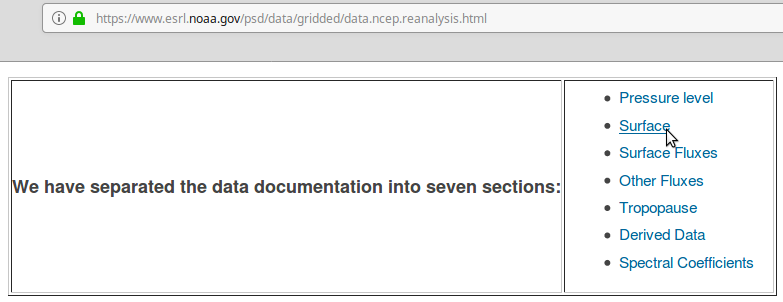
\includegraphics[scale=0.40]{figures/selectingSurfaceSection.png}
							\caption{Selecting \textit{\textbf{Surface}} section.}
							\label{fig:selectingSurfaceSection}
						\end{figure}
					\item \textit{\textbf{Step 3}}: Navigate to the \textit{\textbf{Update Schedule}} section, search for the statistic \textit{\textbf{4-times Daily}} of the desired variable and click on the image for creating a plot or subset (see Fig. \ref{fig:selectingVariable}).
						\begin{figure}[ht!]
							\centering
							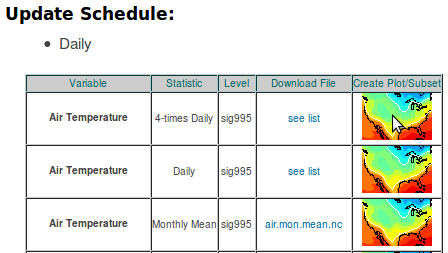
\includegraphics[scale=0.55]{figures/selectingVariable.png}
							\caption{Selecting reanalysis variable.}
							\label{fig:selectingVariable}
						\end{figure}
					\item \textit{\textbf{Step 4}}: Navigate to the \textit{\textbf{Surface}} level and click on \textit{\textbf{Make plot or subset}} (see Fig. \ref{fig:selectingMakePlot}).
						\begin{figure}[ht!]
							\centering
							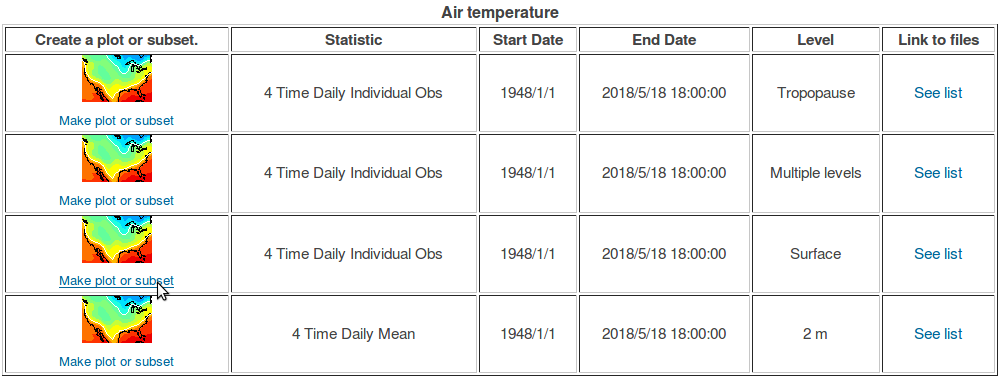
\includegraphics[scale=0.42]{figures/selectingMakePlot.png}
							\caption{Selecting \textit{\textbf{Make plot or subset}.}}
							\label{fig:selectingMakePlot}
						\end{figure}
					\item \textit{\textbf{Step 5}}: In the new web page that has been appeared do the following (see Fig. \ref{fig:selectingProperties.png}):
						\begin{itemize}
							\item In \textit{\textbf{Axis Dimensions}} type the desired sub-grid (spatial properties).
							\item In \textit{\textbf{Other dimension value(s)}} type the desired ranges of dates (temporal properties).
							\item In \textit{\textbf{Output options}} select the option \textit{Create a subset without making a plot}.
							\item Click on \textit{\textbf{Create Plot or Subset of Data}} button (at bottom of the web page) to generate the reanalysis data file with the desired properties.
						\end{itemize}
% 						\begin{figure}[ht!]
% 							\centering
% 							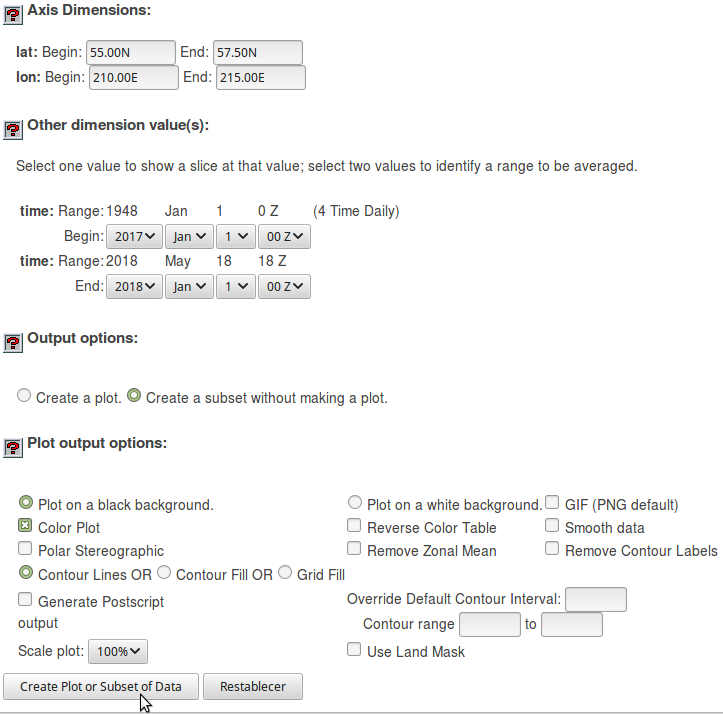
\includegraphics[scale=0.50]{figures/selectingProperties.png}
% 							\caption{Typing desired properties of the file to get.}
% 							\label{fig:selectingProperties.png}
% 						\end{figure}
					\item \textit{\textbf{Step 6}}: Finally click on \textit{\textbf{FTP a copy of the file}} button to download the reanalysis data file on the computer.
				\end{itemize}
				
				\begin{figure}[ht!]
					\centering
					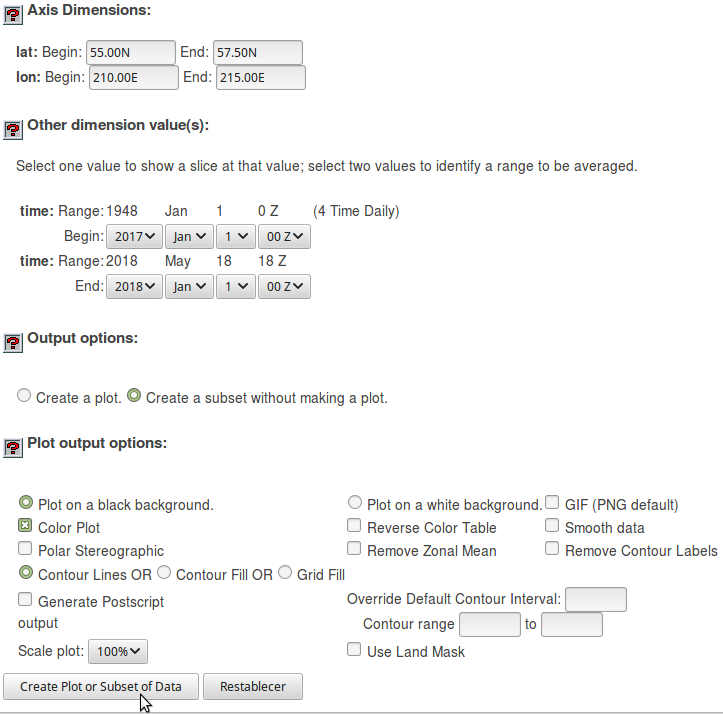
\includegraphics[scale=0.50]{figures/selectingProperties.png}
					\caption{Typing desired properties of the file to get.}
					\label{fig:selectingProperties.png}
				\end{figure}
				
				\clearpage
				
	\end{onehalfspace}
	
%	Formato abreviado:

%	Follow these steps to obtain an annual text file that contain the measurements collected by a buoy from NDBC:
%		\begin{itemize}
%			\item \textit{\textbf{Step 1}}: Open the web browser and visit the NDBC web page \cite{NOAA_1}.
%			\item \textit{\textbf{Step 2}}: Navigate to the desired buoy and click on the year to download.
%			\item \textit{\textbf{Step 3}}: In the option \textit{\textbf{Method Two}} click on the file and its content will be shown.
%			\item \textit{\textbf{Step 4}}: In the menu bar of the web browser select \textit{\textbf{File}} and \textit{\textbf{Save As}} to save it in the computer.
%		\end{itemize}	

%	Formato abreviado:
		
%	Follow these steps to obtain a reanalysis data file from NNRP:
%	
%		\begin{itemize}
%			\item \textit{\textbf{Step 1}}: Open the web browser and visit the NNRP  web page \cite{NNRP}.
%			\item \textit{\textbf{Step 2}}: Navigate to the \textit{\textbf{Surface}} section and click on it.
%			\item \textit{\textbf{Step 3}}: Navigate to the \textit{\textbf{Update Schedule}} section, search for the statistic \textit{\textbf{4-times Daily}} of the desired variable and click on the image for creating a plot or subset.
%			\item \textit{\textbf{Step 4}}: Navigate to the \textit{\textbf{Surface}} level and click on \textit{\textbf{Make plot or subset}}.
%			\item \textit{\textbf{Step 5}}: In the new web page that has been appeared do the following:
%				\begin{itemize}
%					\item In \textit{\textbf{Axis Dimensions}} type the desired grid (spatial properties).
%					\item In \textit{\textbf{Other dimension value(s)}} type the desired ranges of dates (temporal properties).
%					\item In \textit{\textbf{Output options}} select the option \textit{Create a subset without making a plot}.
%					\item Click on \textit{\textbf{Create Plot or Subset of Data}} button (bottom of the web page) to generate the reanalysis data file with the desired properties.
%				\end{itemize}
%			\item \textit{\textbf{Step 6}}: Finally click on \textit{\textbf{FTP a copy of the file}} button to download the reanalysis data file on the computer.
%		\end{itemize}
